\section{Benchmarks}

\subsection{Benchmark 1: RC Anti-Aliasing}

The first benchmark is a textbook ECG-style RC low-pass filter before a 500 Hz ADC. CiTT parsed the problem, built/opened a Simscape model, produced teaching and probe evidence, and generated Bode plots. The live report records $R=39.8~\mathrm{k\Omega}$, $C=100~\mathrm{nF}$, $\tau=0.00398~\mathrm{s}$, $f_c=39.9887~\mathrm{Hz}$, and 60 Hz attenuation of $-5.1205~\mathrm{dB}$.

\begin{figure*}[t]
\centering
\begin{tabular}{ccc}
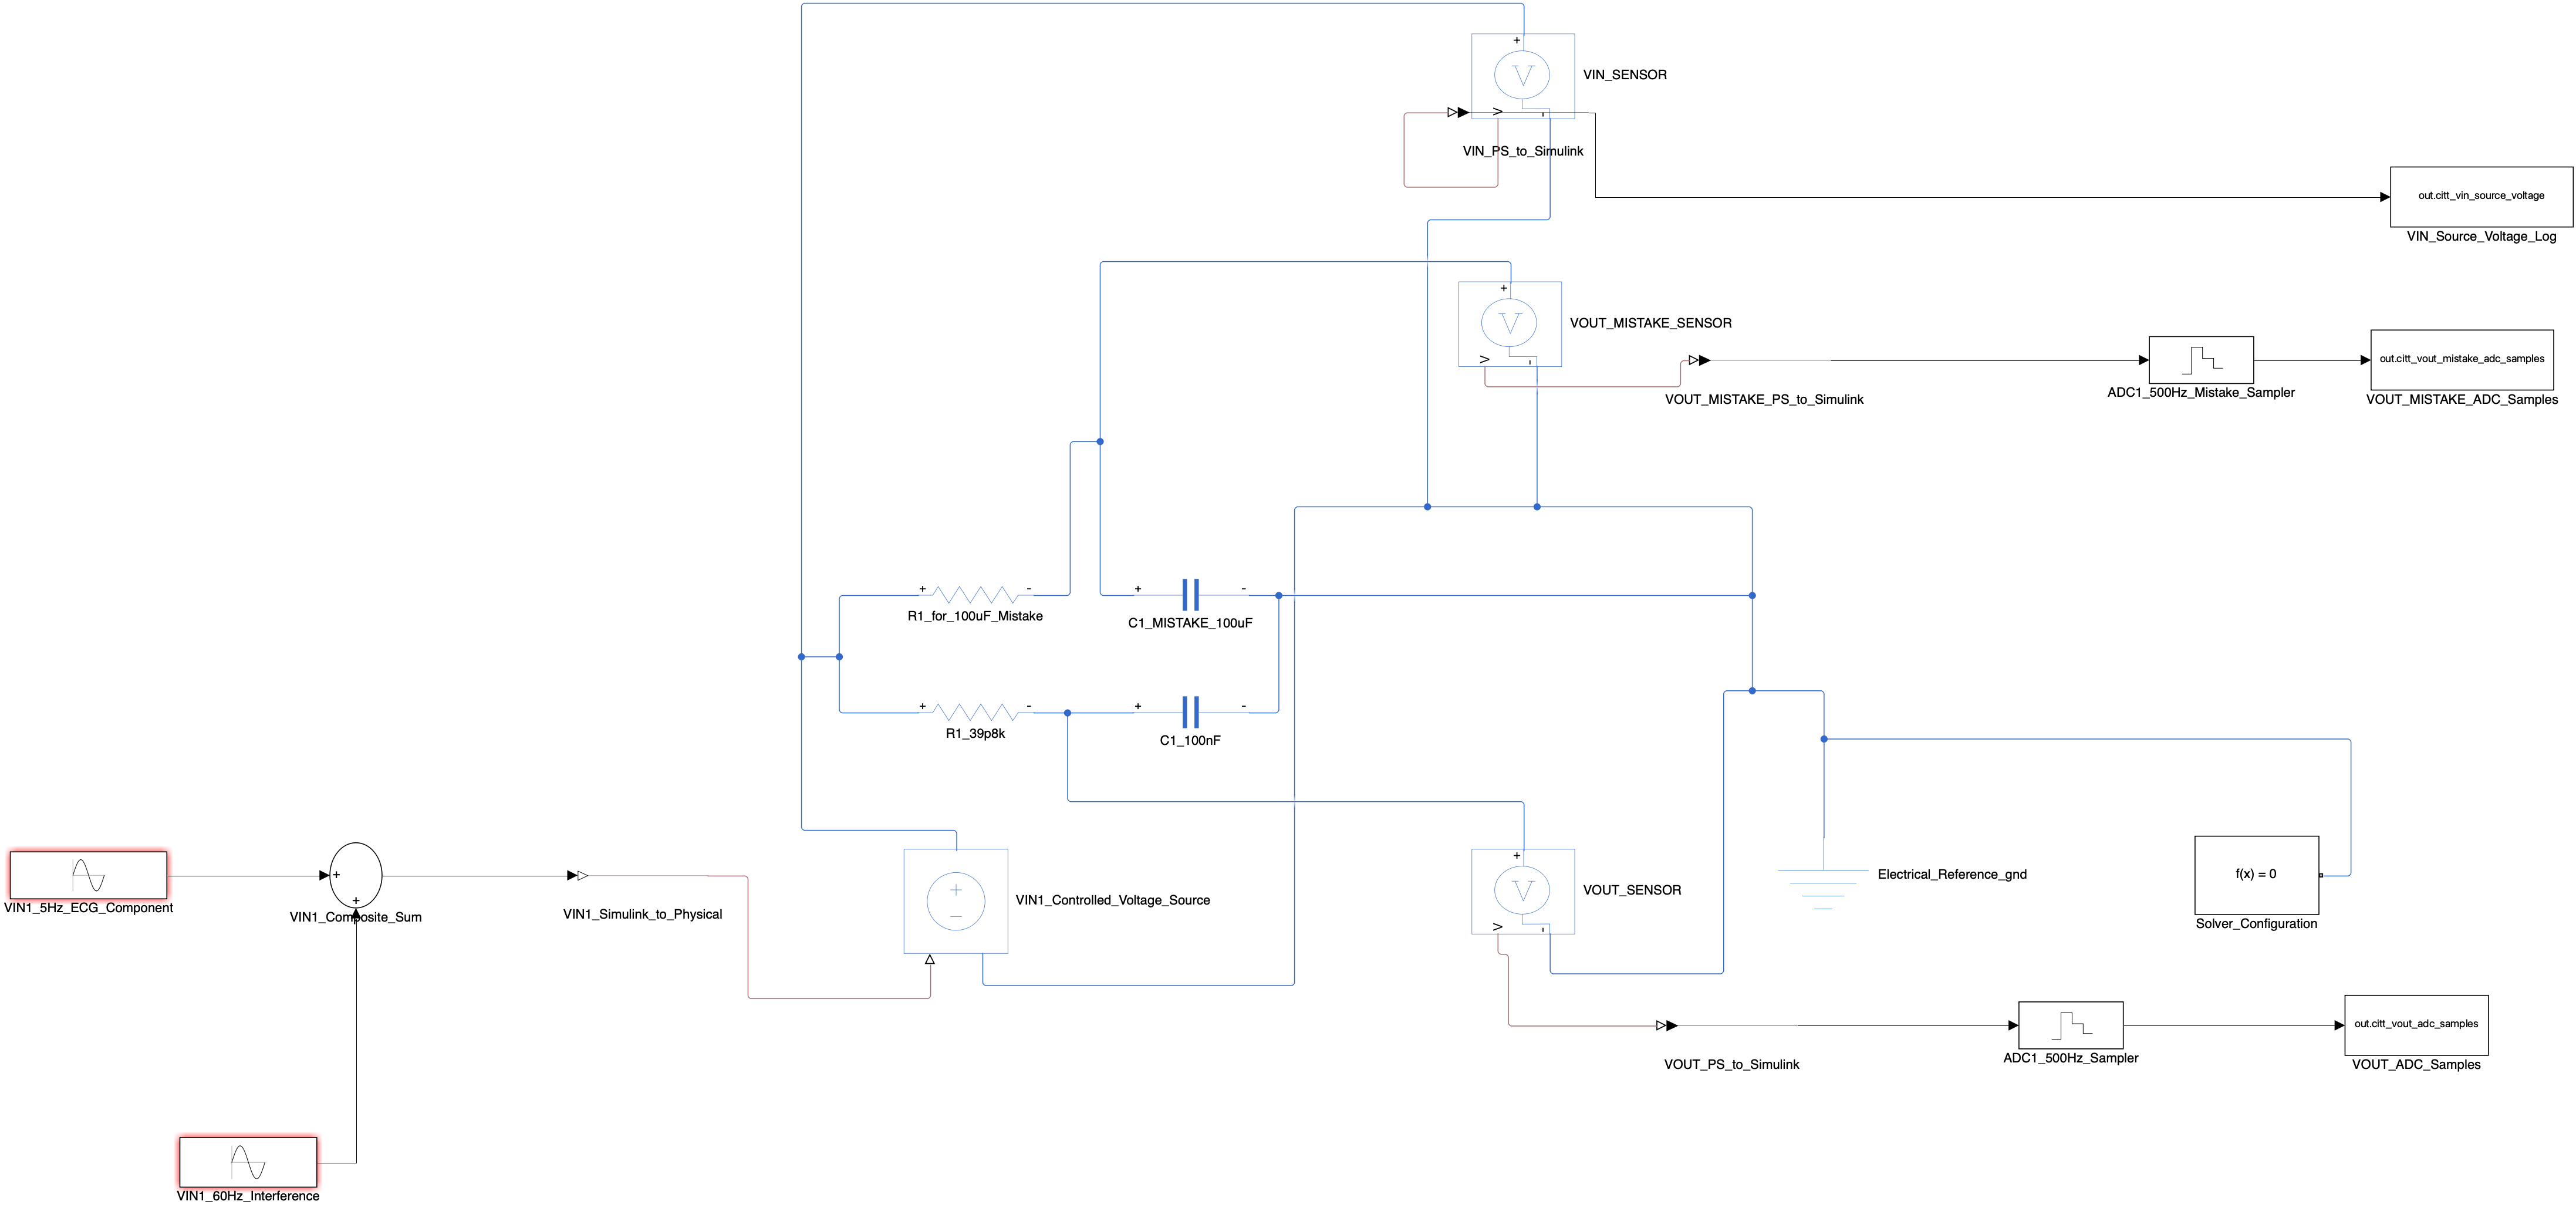
\includegraphics[width=0.31\textwidth]{figures/fig3_rc_model.png} &
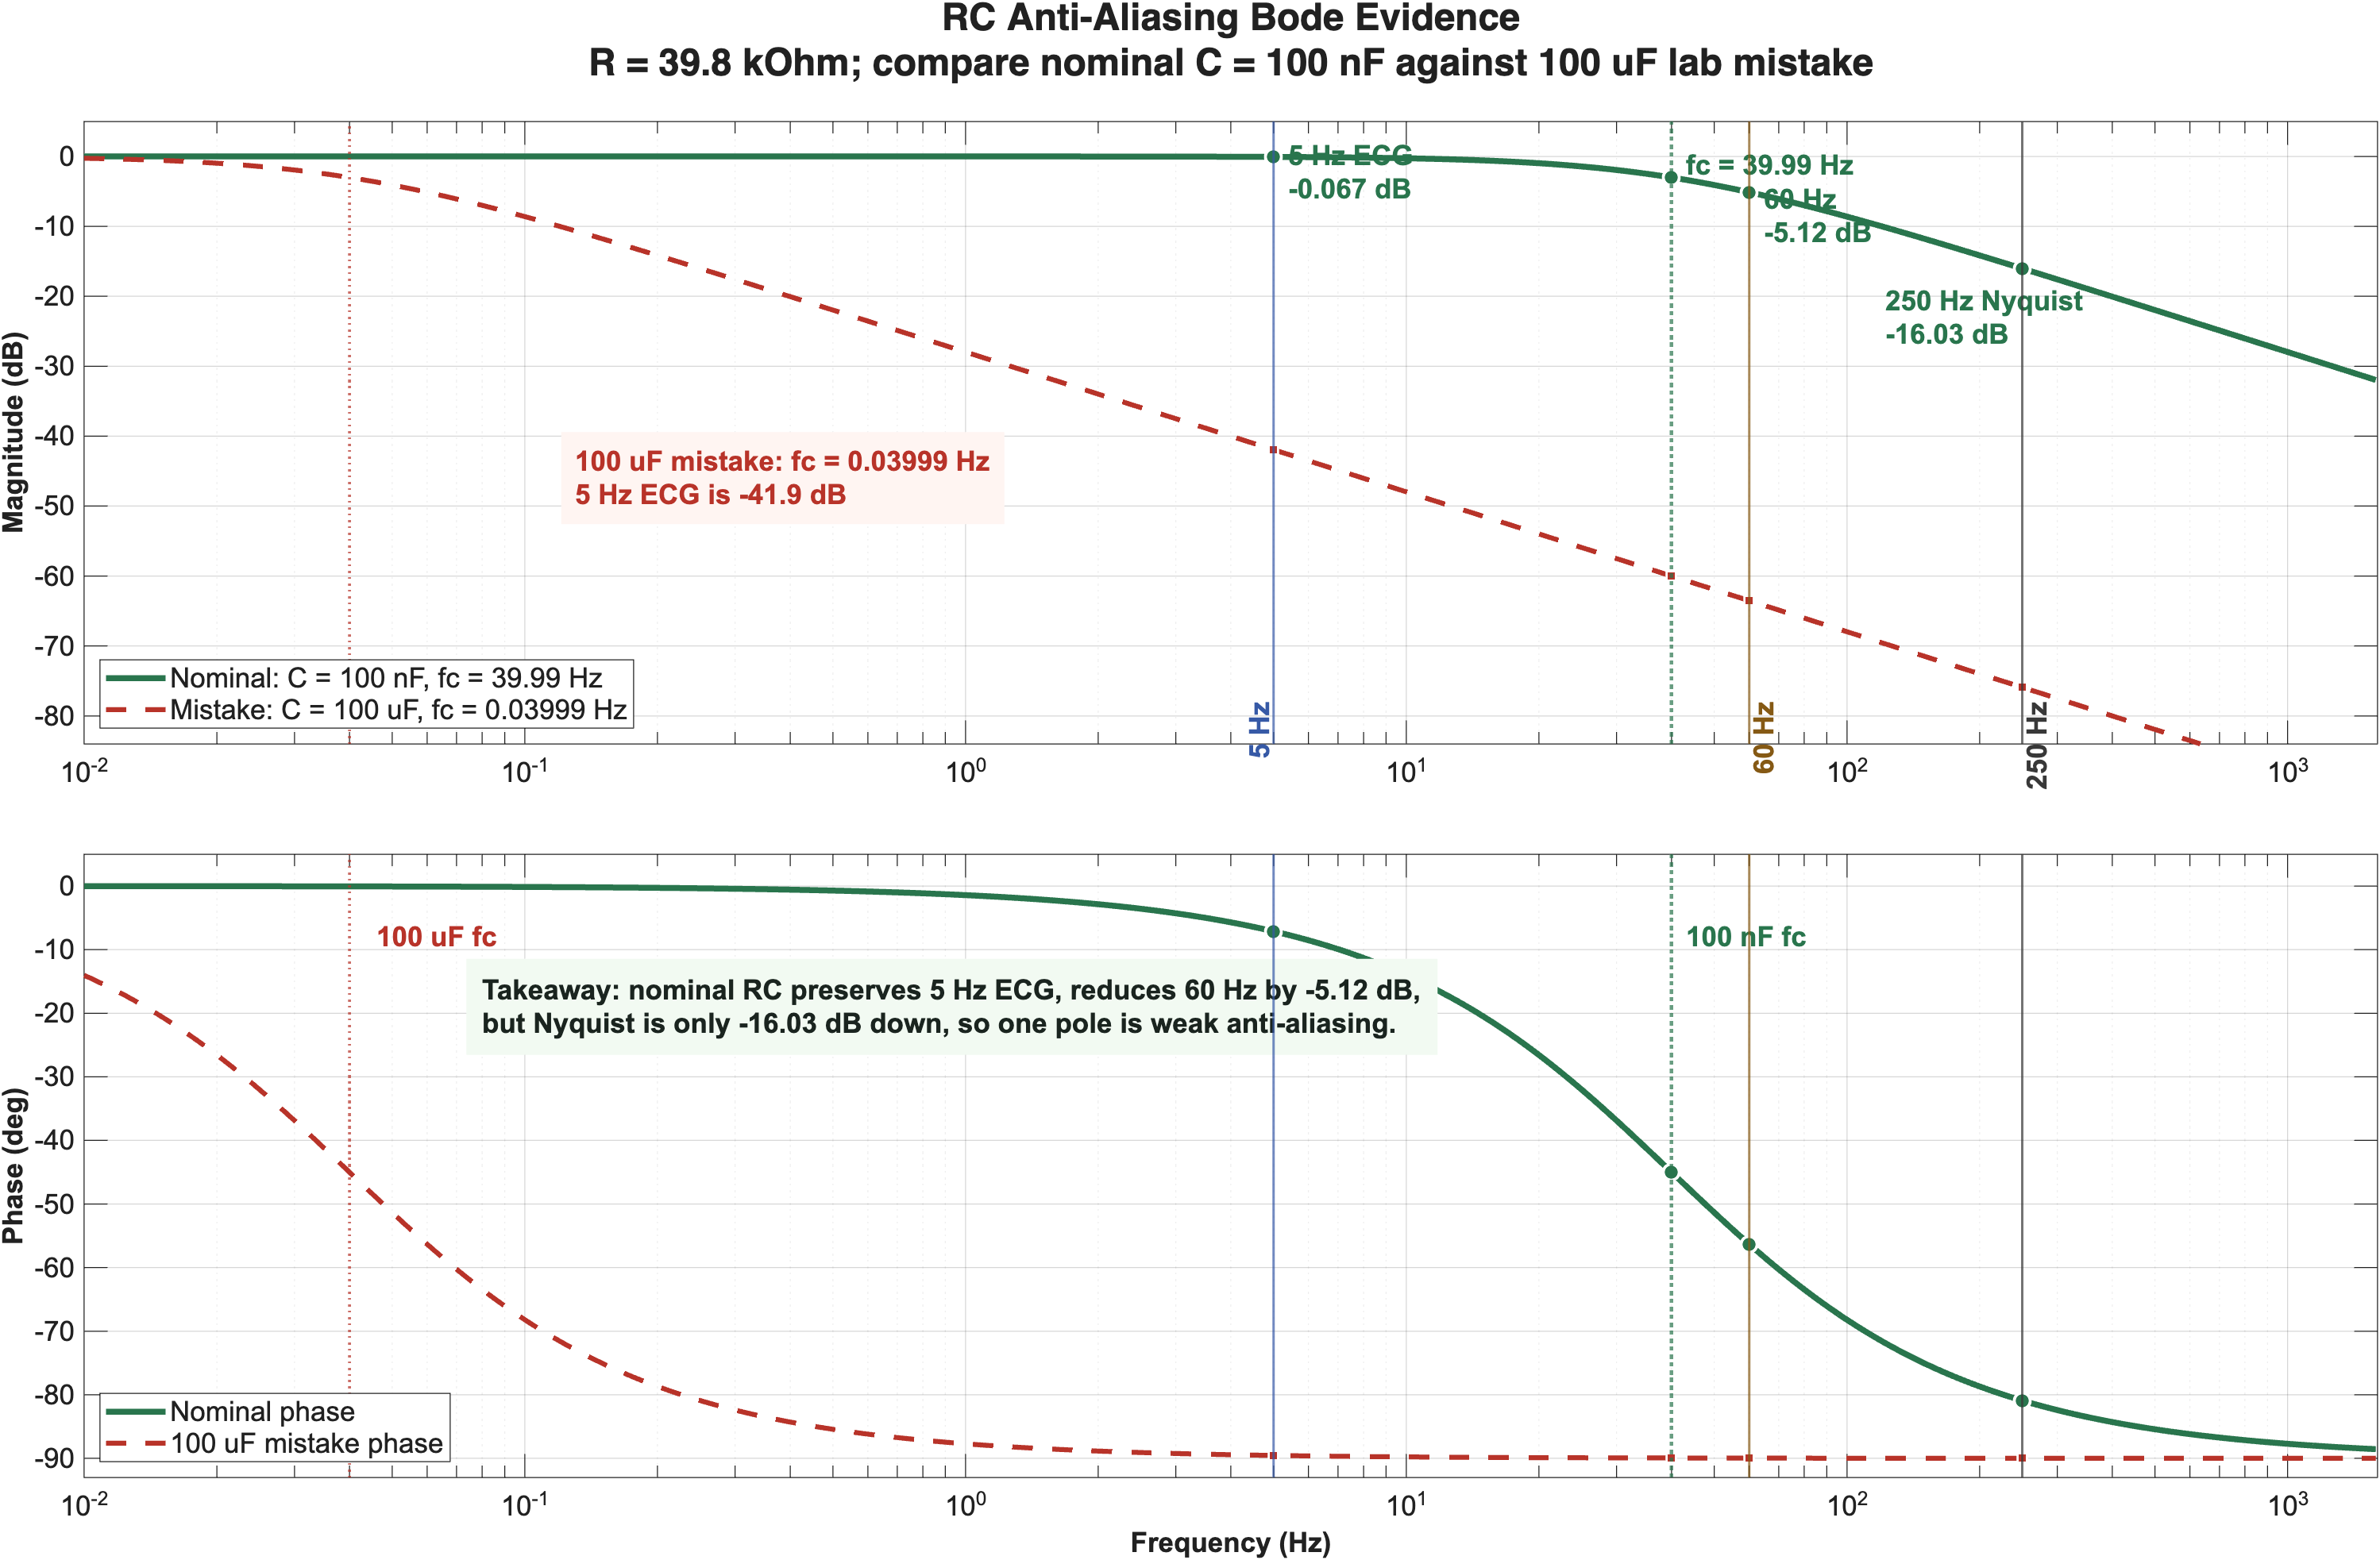
\includegraphics[width=0.31\textwidth]{figures/fig3_rc_bode.png} &
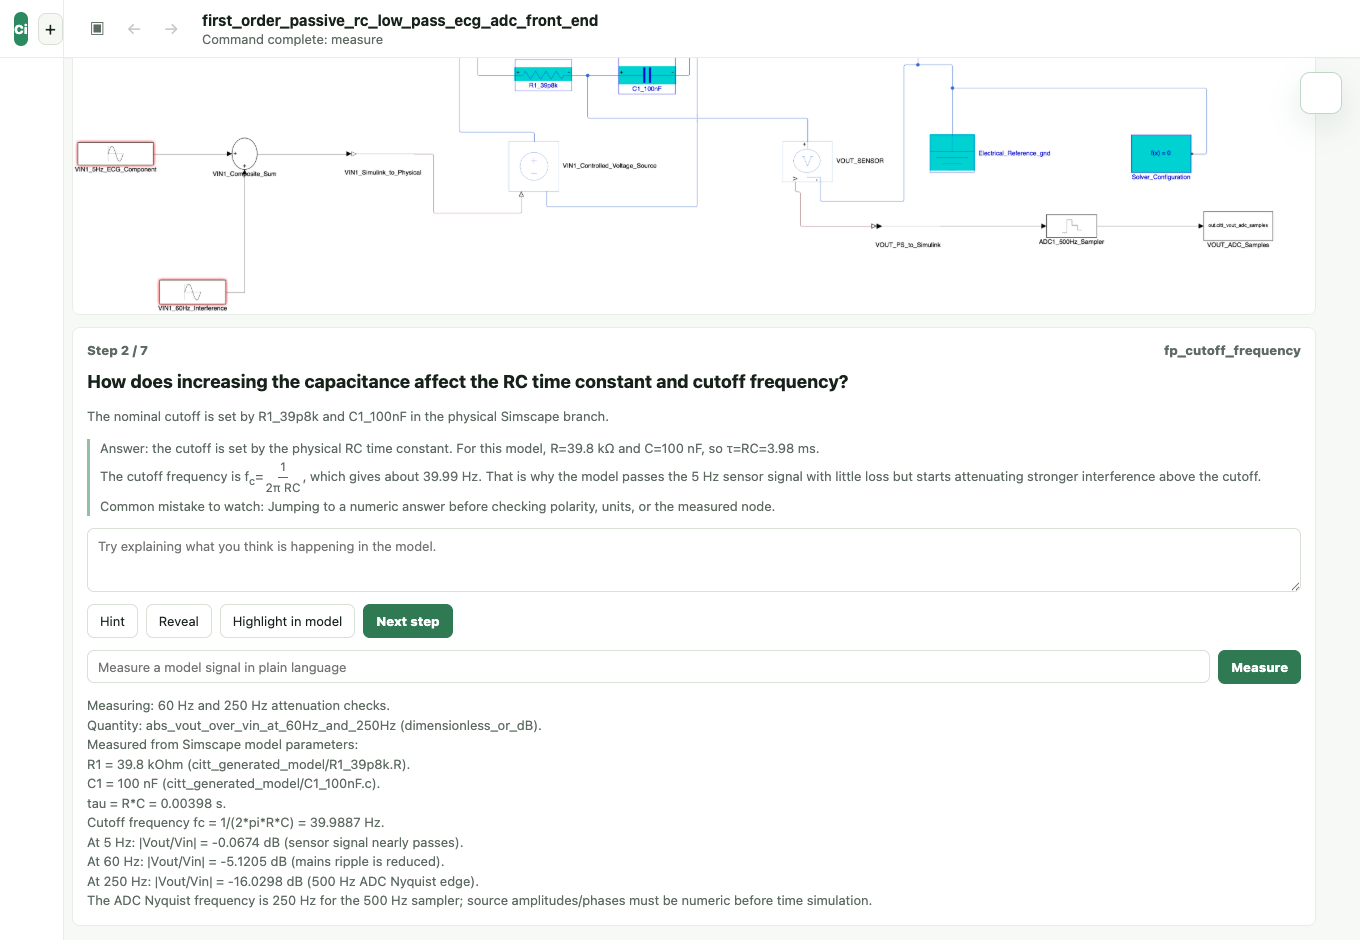
\includegraphics[width=0.31\textwidth]{figures/fig3_rc_probe.png} \\
(a) Simscape model & (b) Bode evidence & (c) Probe output
\end{tabular}
\caption{Benchmark 1 RC evidence. CiTT links textbook calculations to an inspectable model, annotated frequency response, and natural-language probe evidence.}
\label{fig:rc}
\end{figure*}

\subsection{Benchmark 2: TEVC Equilibrium}

The second benchmark is a simplified two-electrode voltage clamp equivalent circuit. CiTT generated a Simscape-first electrical model with command source, buffer path, finite-gain amplifier, $R_o$, $R_m$, symbolic $R_e$, membrane-voltage probe, amplifier-output probe, clamp-current probe, electrical reference, and solver configuration. $V_c$ and $R_e$ remain symbolic because the benchmark source omits numeric values.

\begin{figure*}[t]
\centering
\begin{tabular}{ccc}
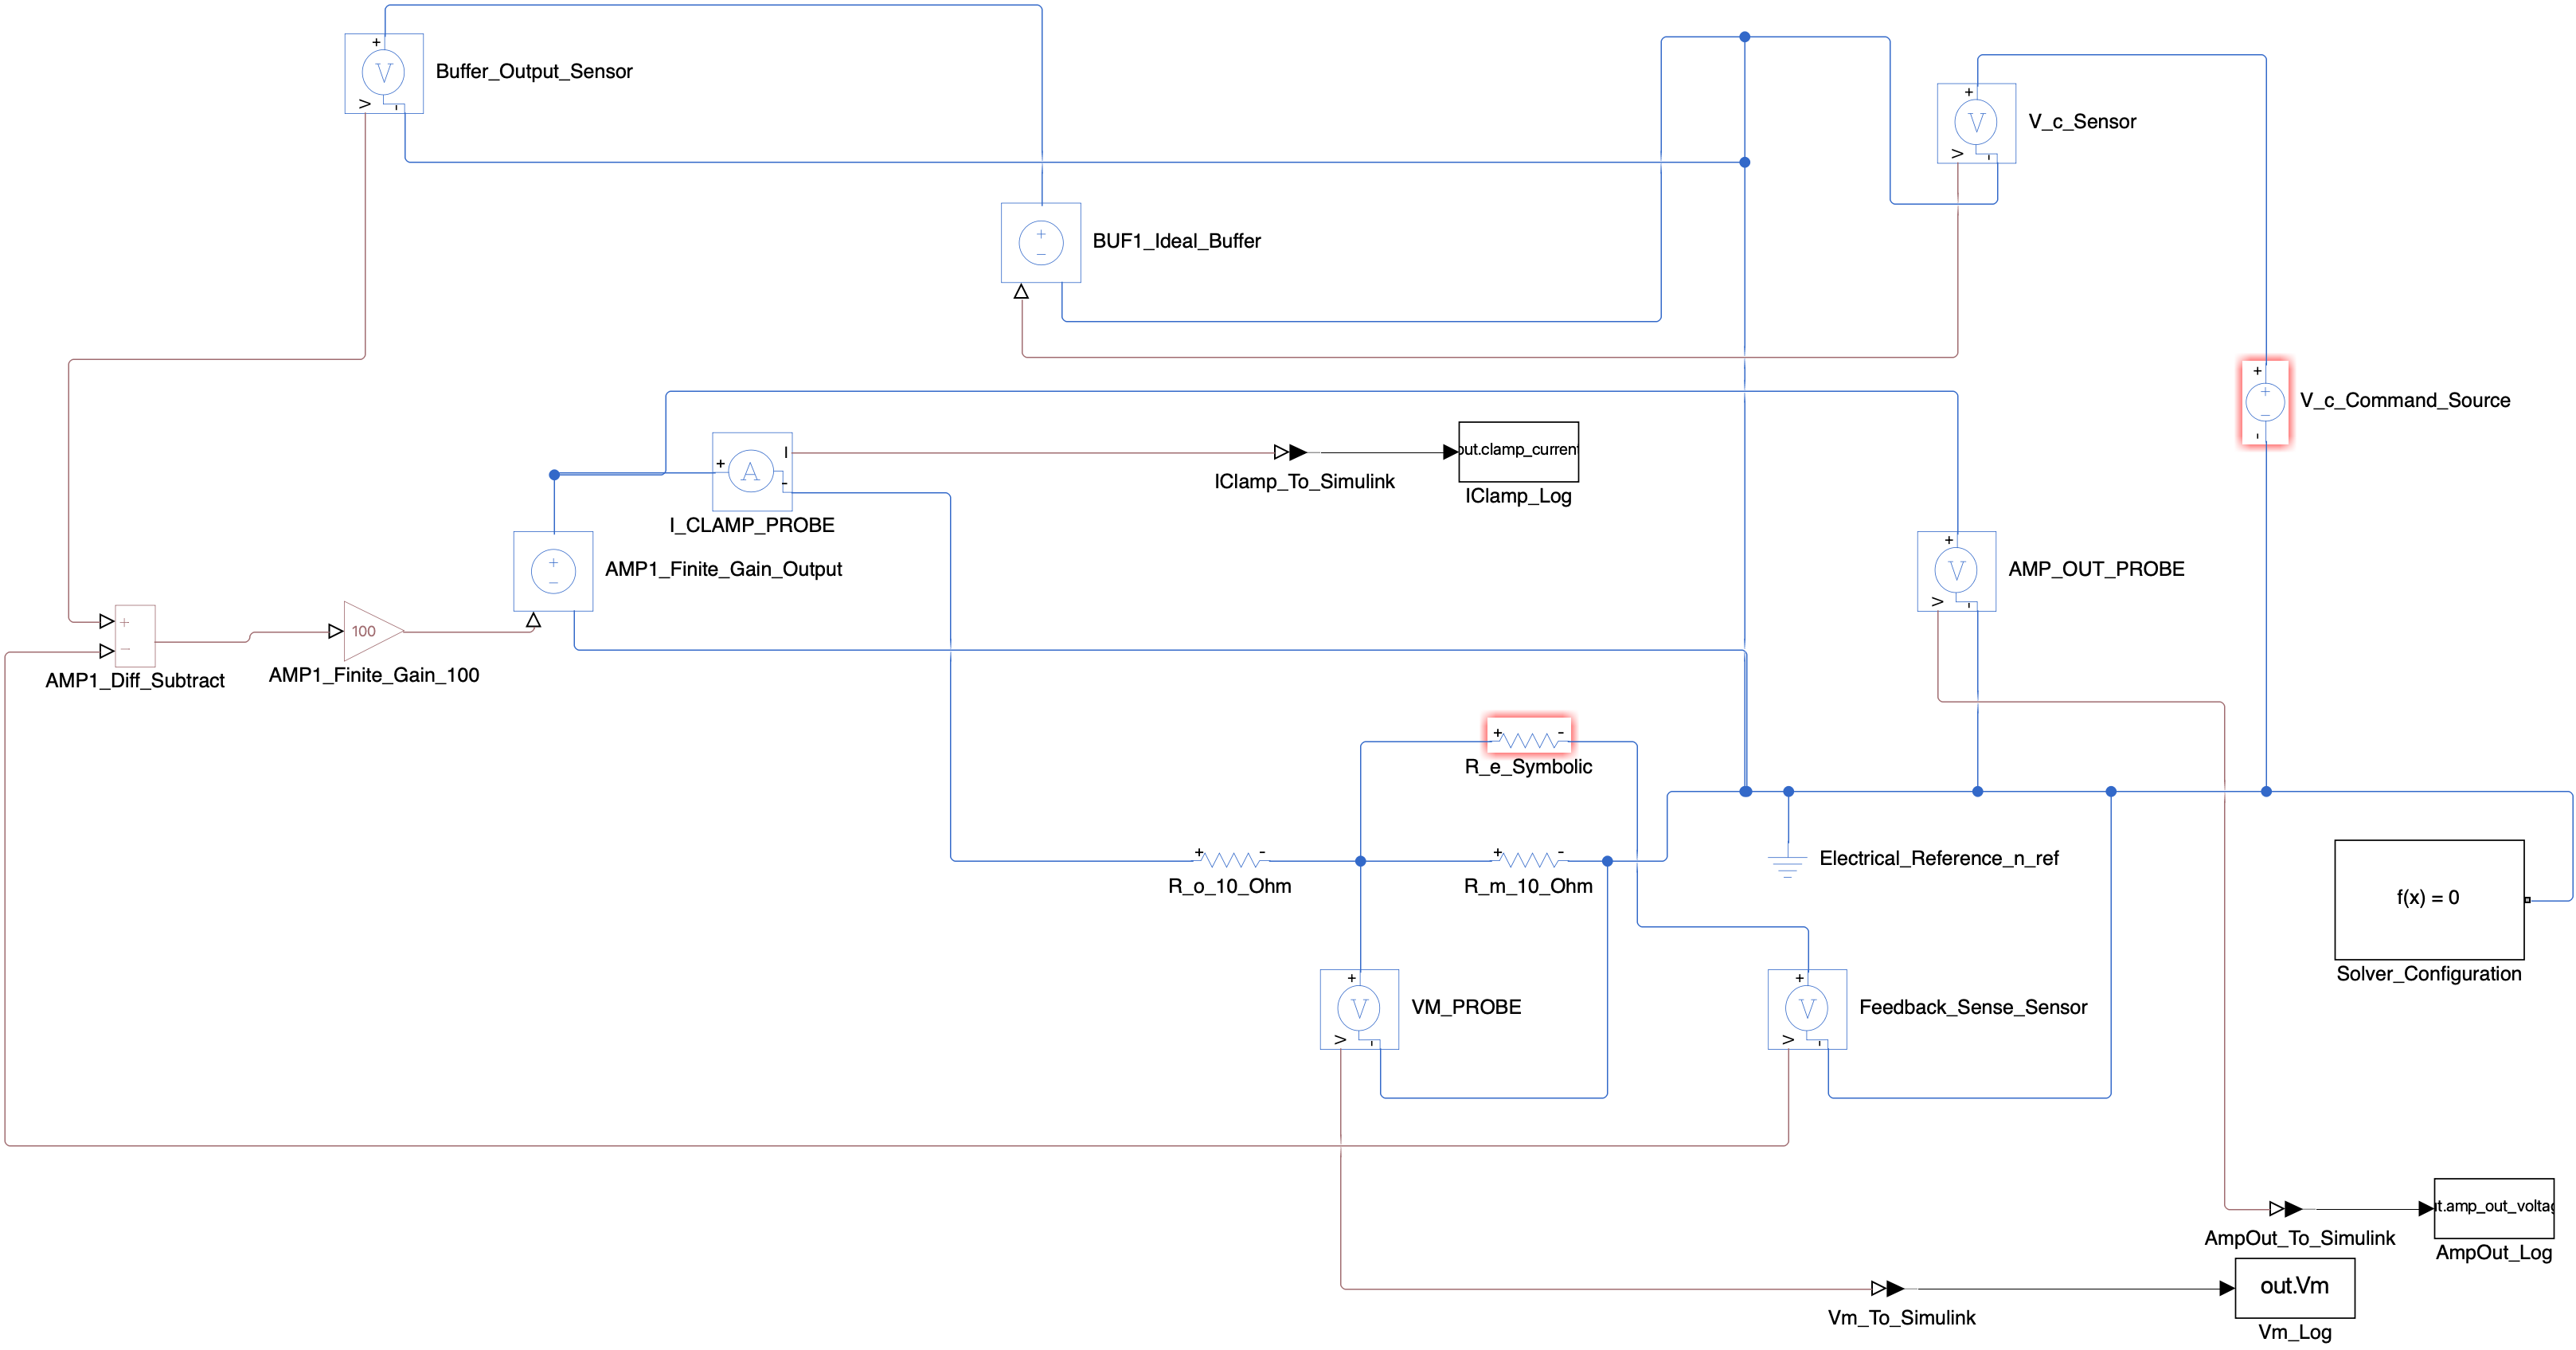
\includegraphics[width=0.31\textwidth]{figures/fig4_tevc_model.png} &
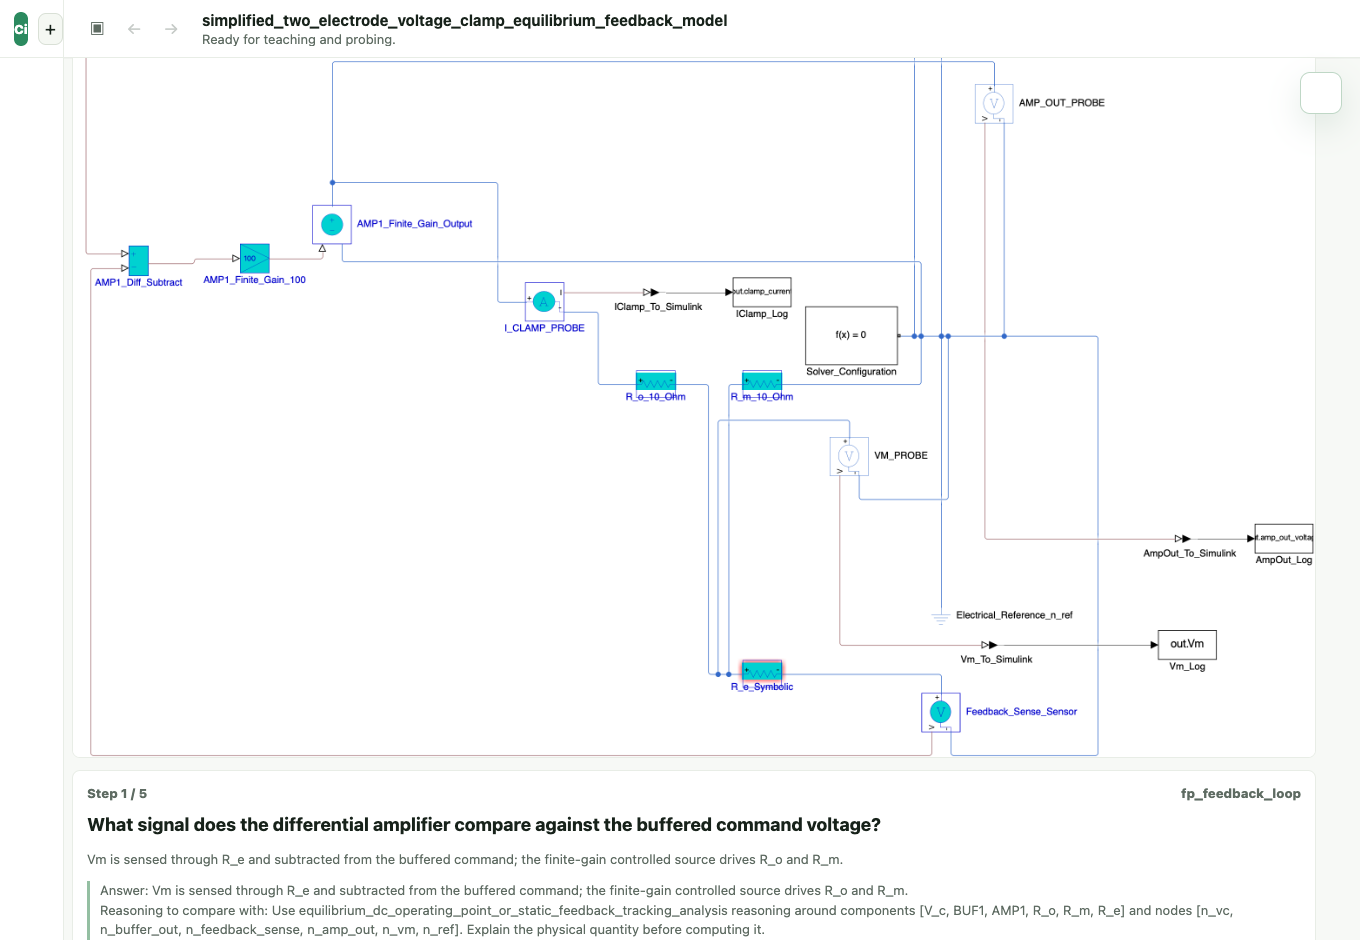
\includegraphics[width=0.31\textwidth]{figures/fig4_tevc_feedback.png} &
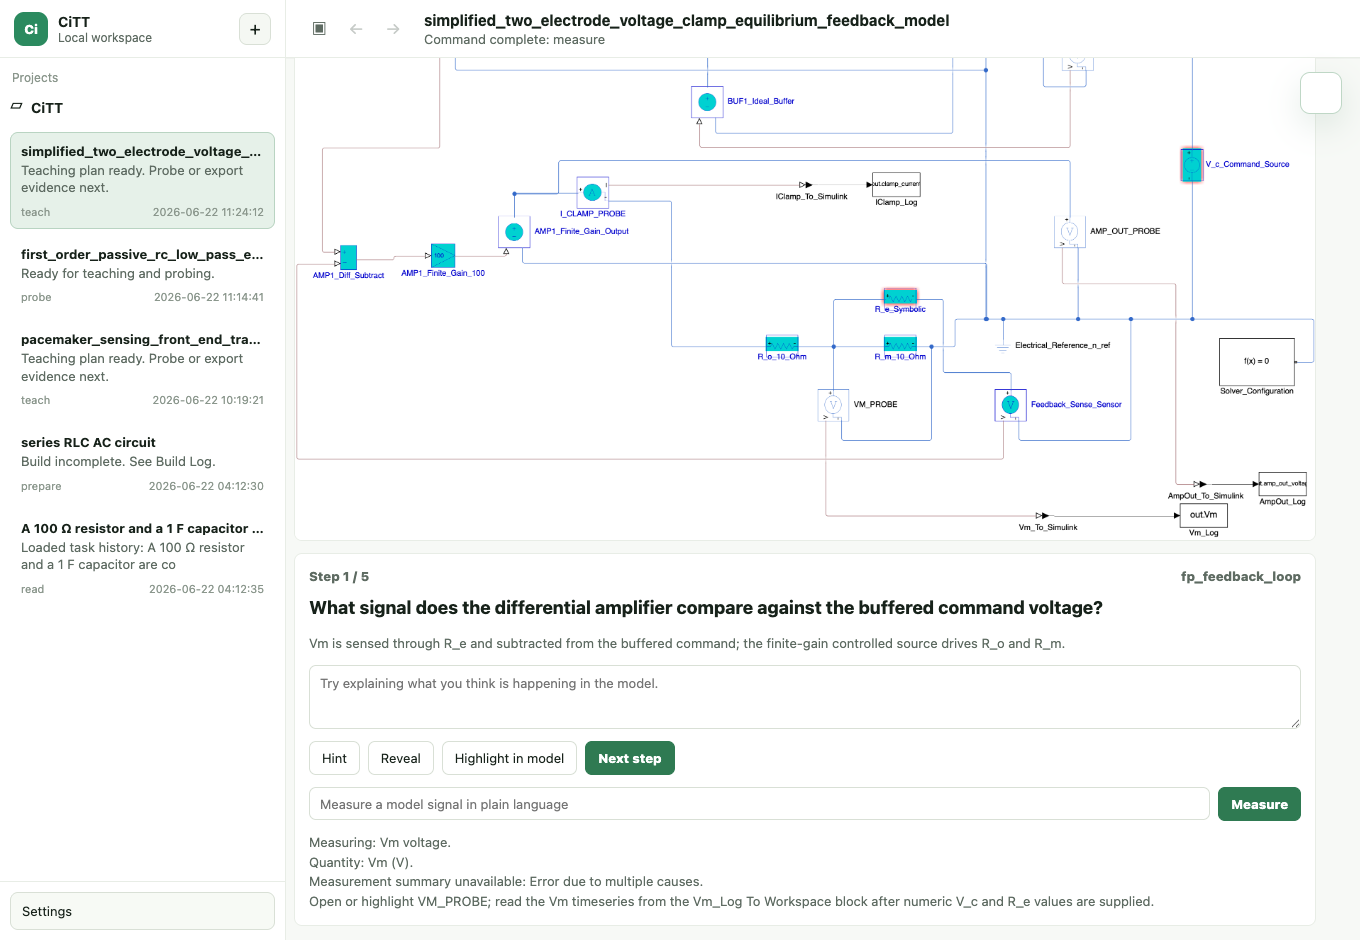
\includegraphics[width=0.31\textwidth]{figures/fig4_tevc_probe.png} \\
(a) Arranged model & (b) Feedback teaching & (c) Chat-style probe
\end{tabular}
\caption{Benchmark 2 TEVC evidence. CiTT preserves symbolic values while linking feedback teaching and probe output to focus/probe maps.}
\label{fig:tevc}
\end{figure*}

\subsection{Benchmark 3: Mixed-Signal Neural Clamp}

The third benchmark is a closed-loop mixed-signal neural-clamp teaching example with membrane dynamics, electrode series resistance, finite-gain/nonideal amplifier behavior, rail and current limits, ADC quantization, digital control state, and fault/parameter-sweep evidence. It uses educational scaled parameters and should be read as model-based learning evidence.

\begin{figure*}[t]
\centering
\begin{tabular}{cc}
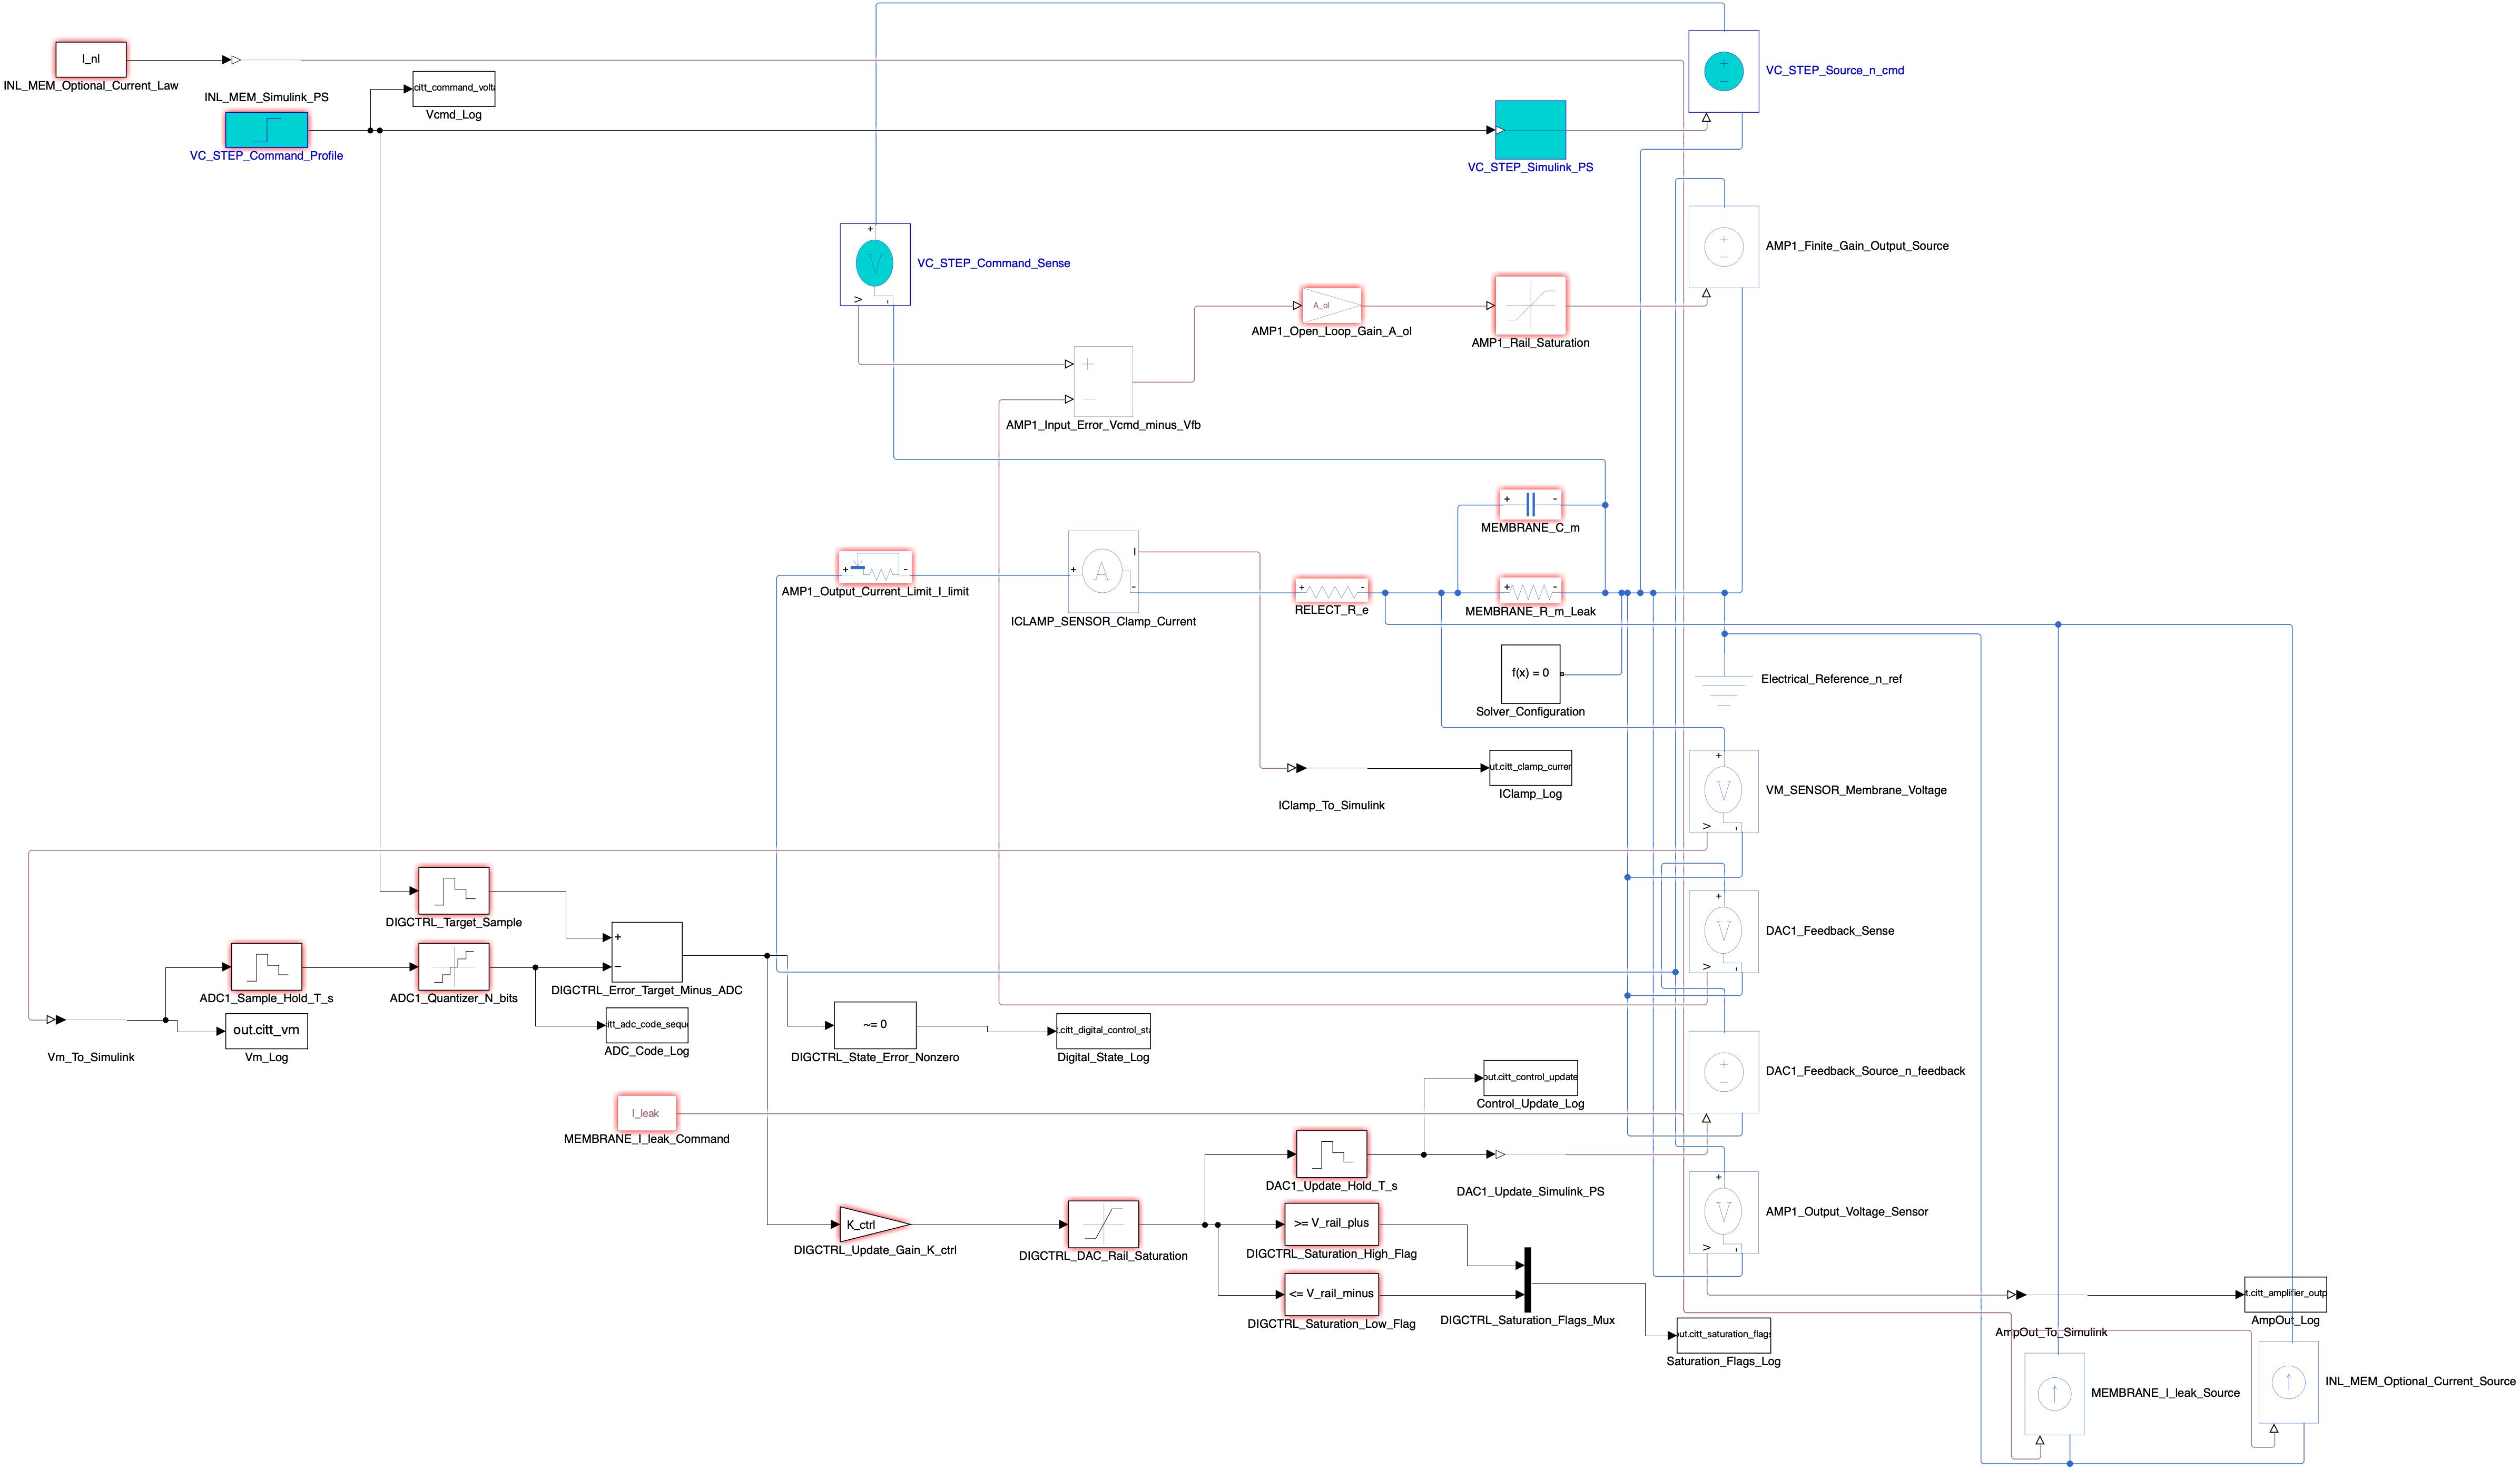
\includegraphics[width=0.47\textwidth]{figures/fig5_mixed_model.png} &
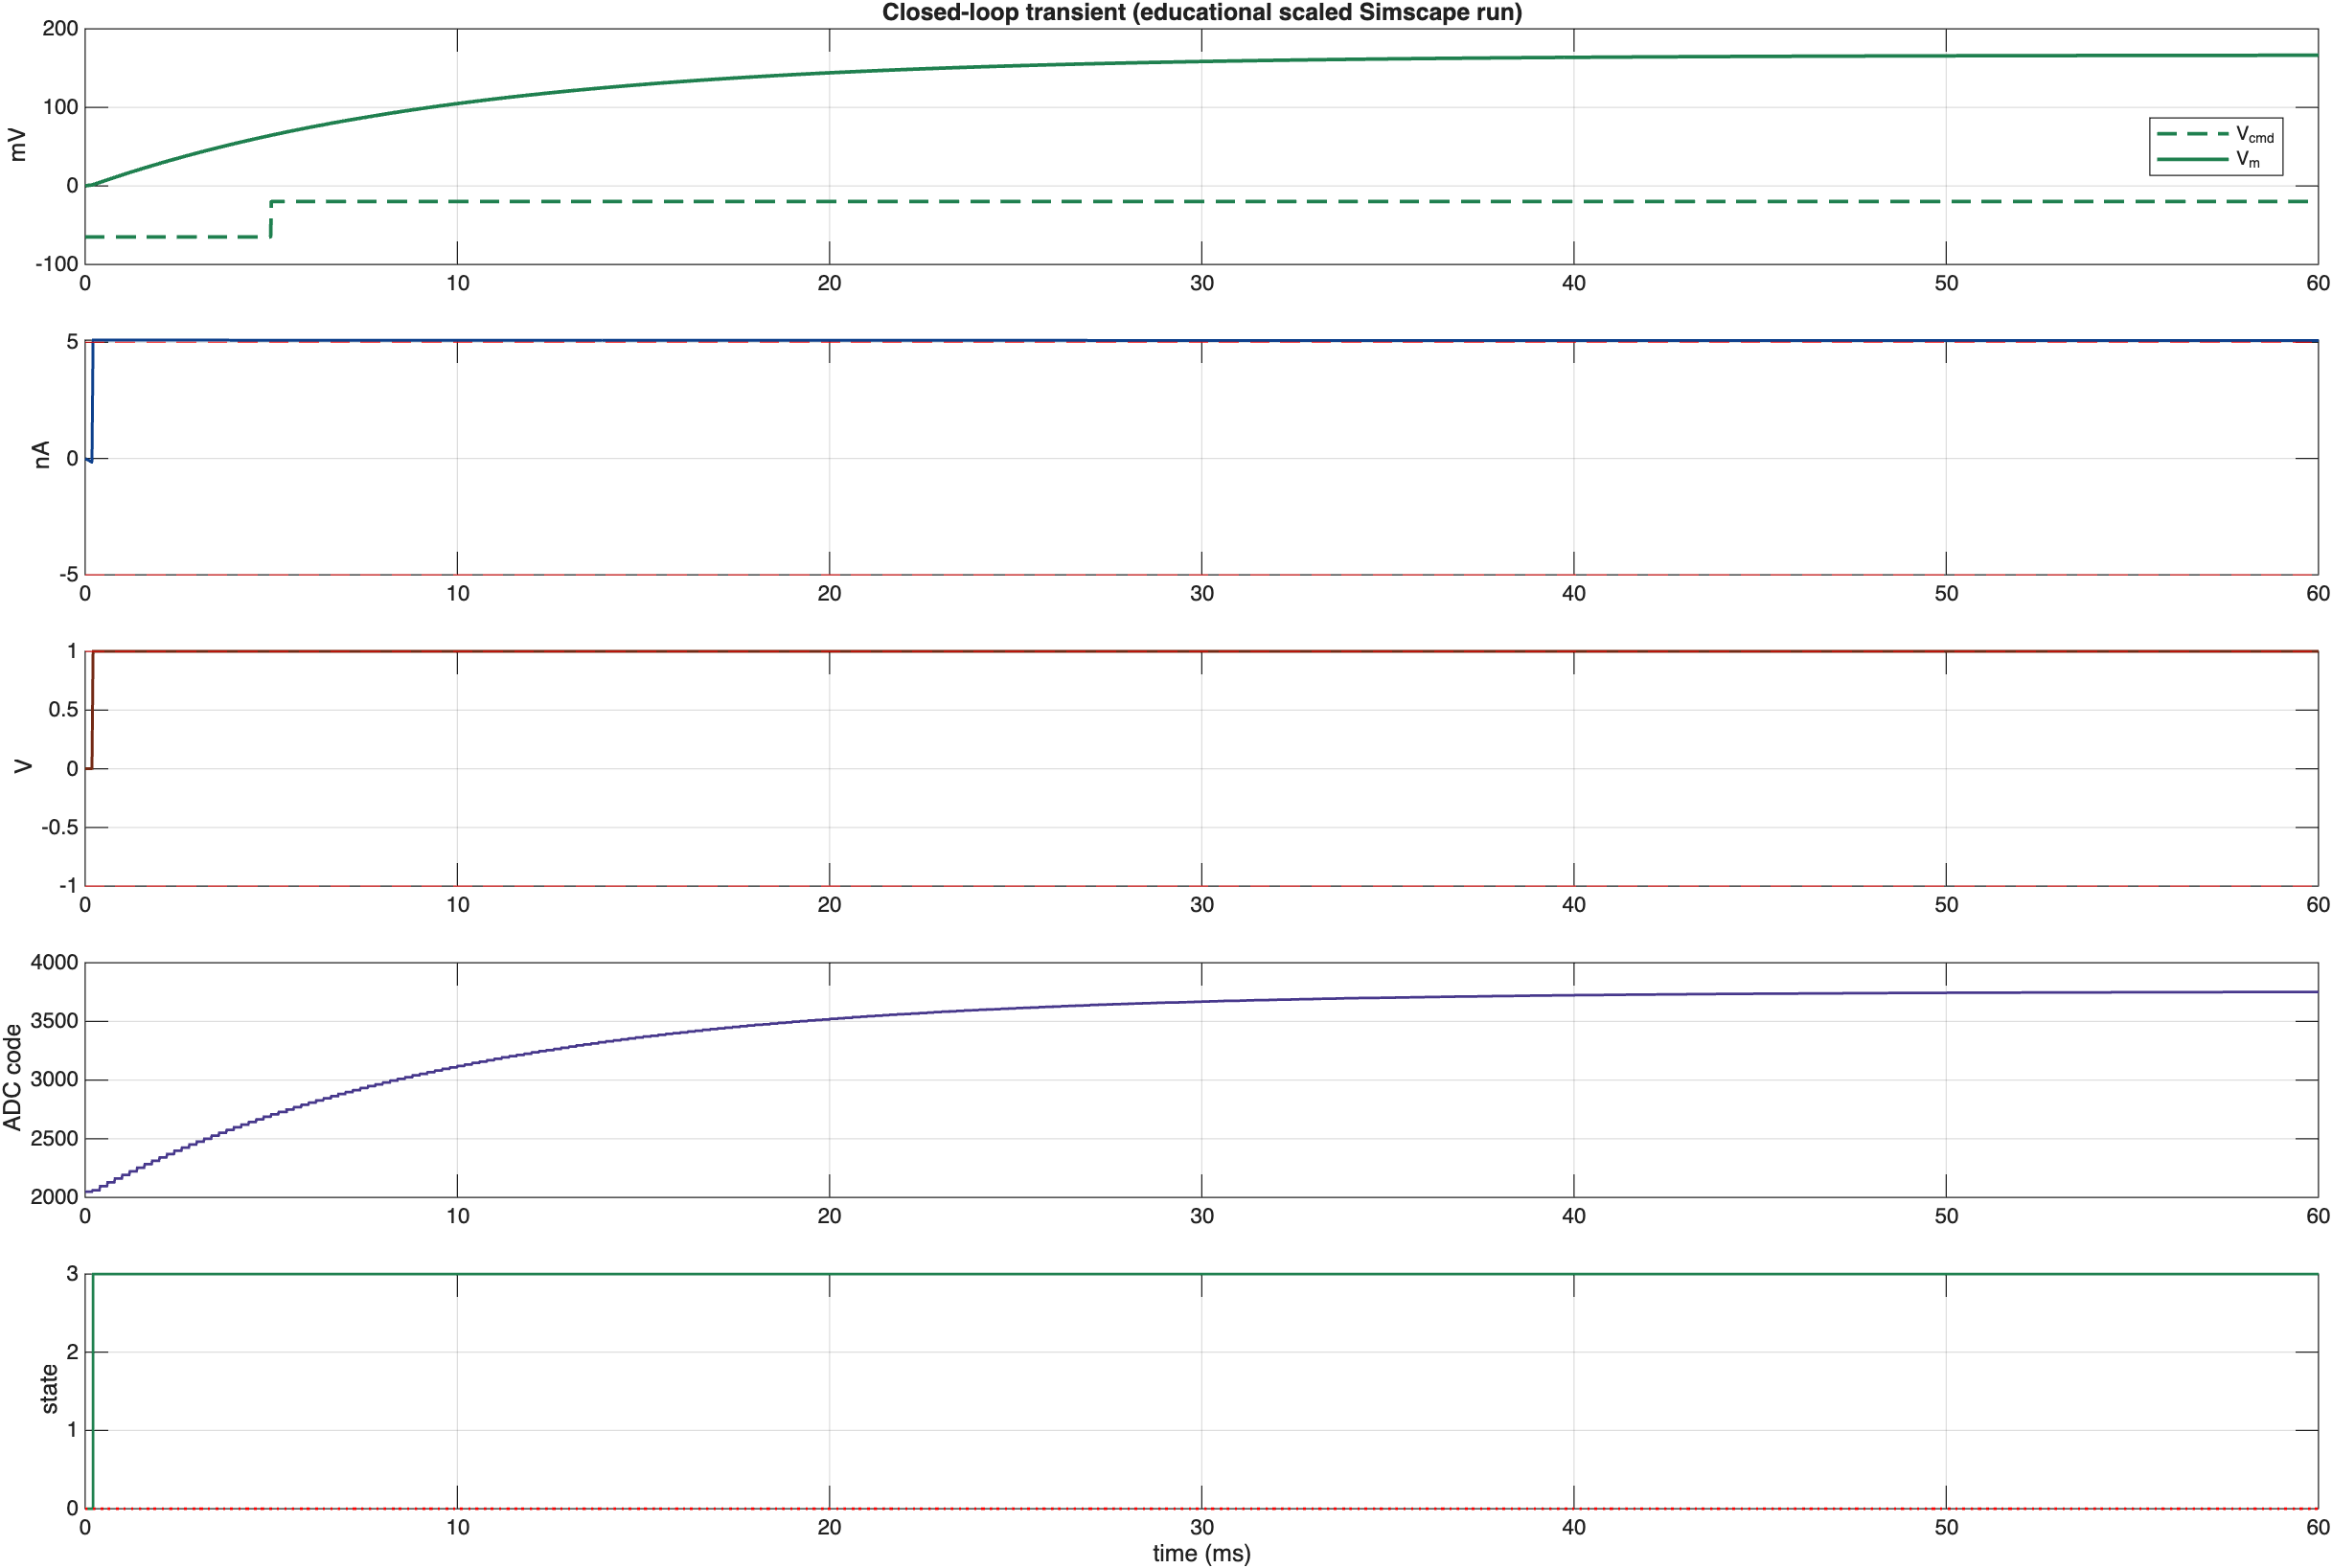
\includegraphics[width=0.47\textwidth]{figures/fig5_mixed_timeline.png} \\
(a) Arranged model & (b) Timeline plot \\
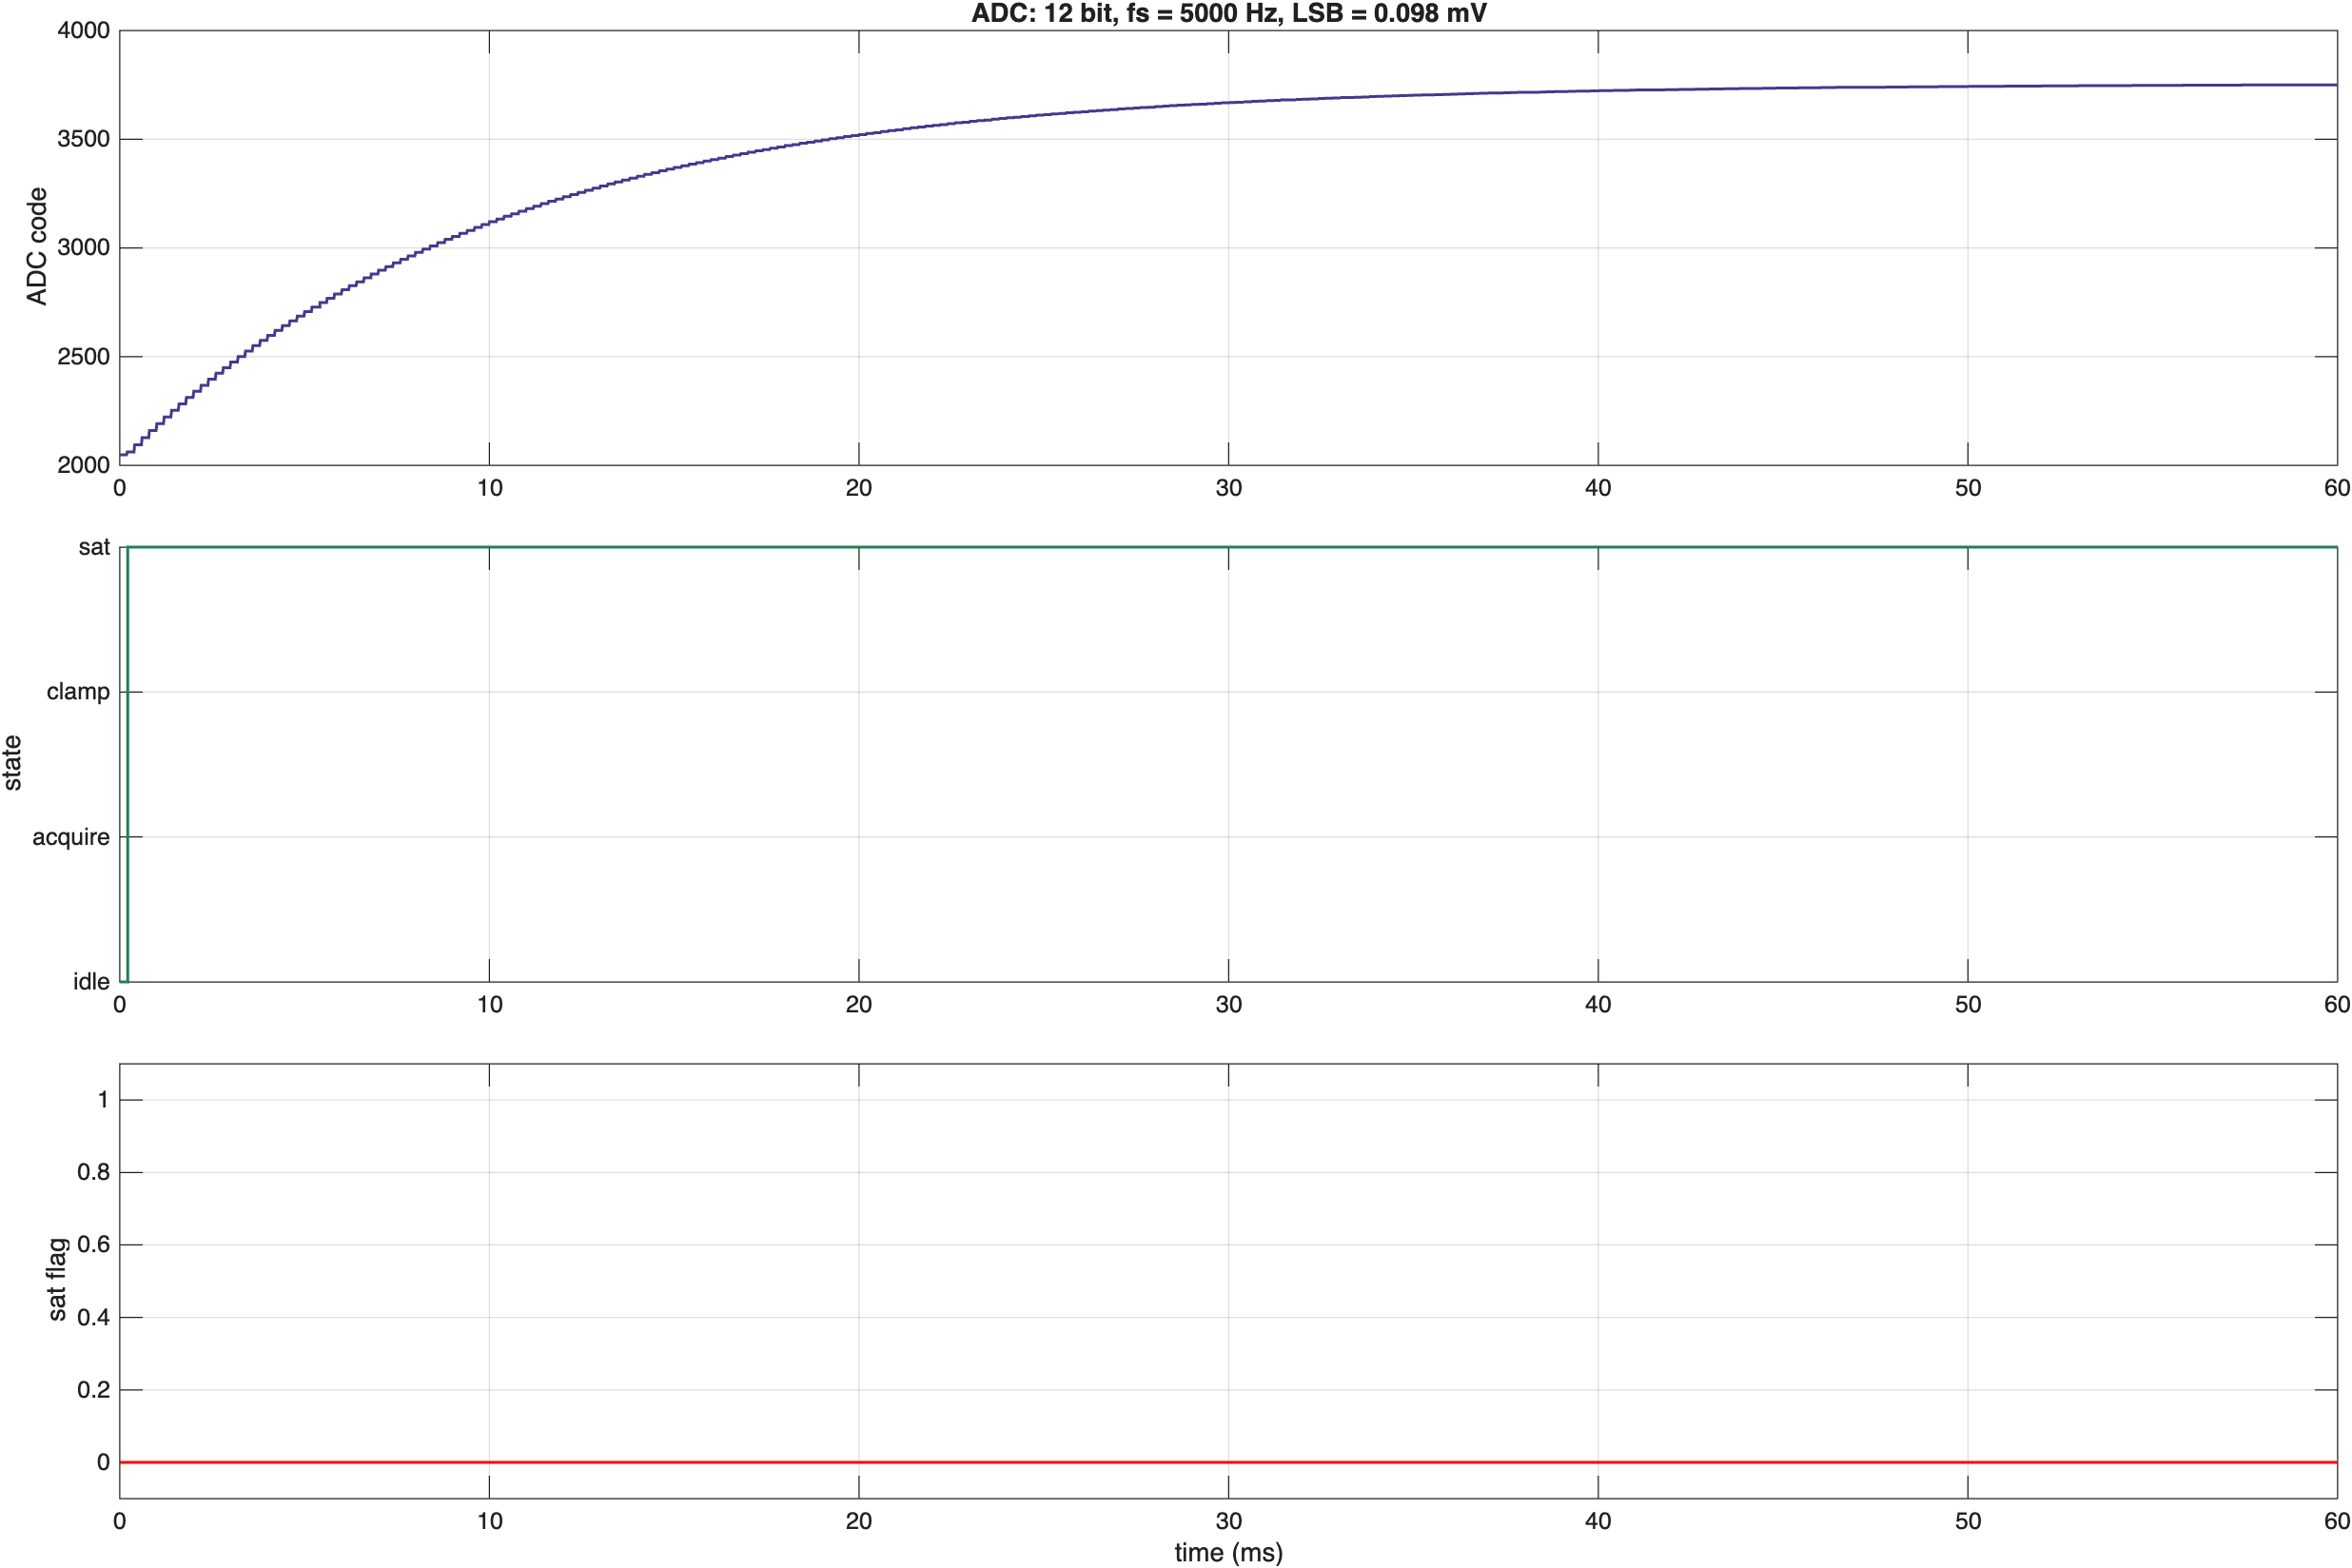
\includegraphics[width=0.47\textwidth]{figures/fig5_mixed_adc.png} &
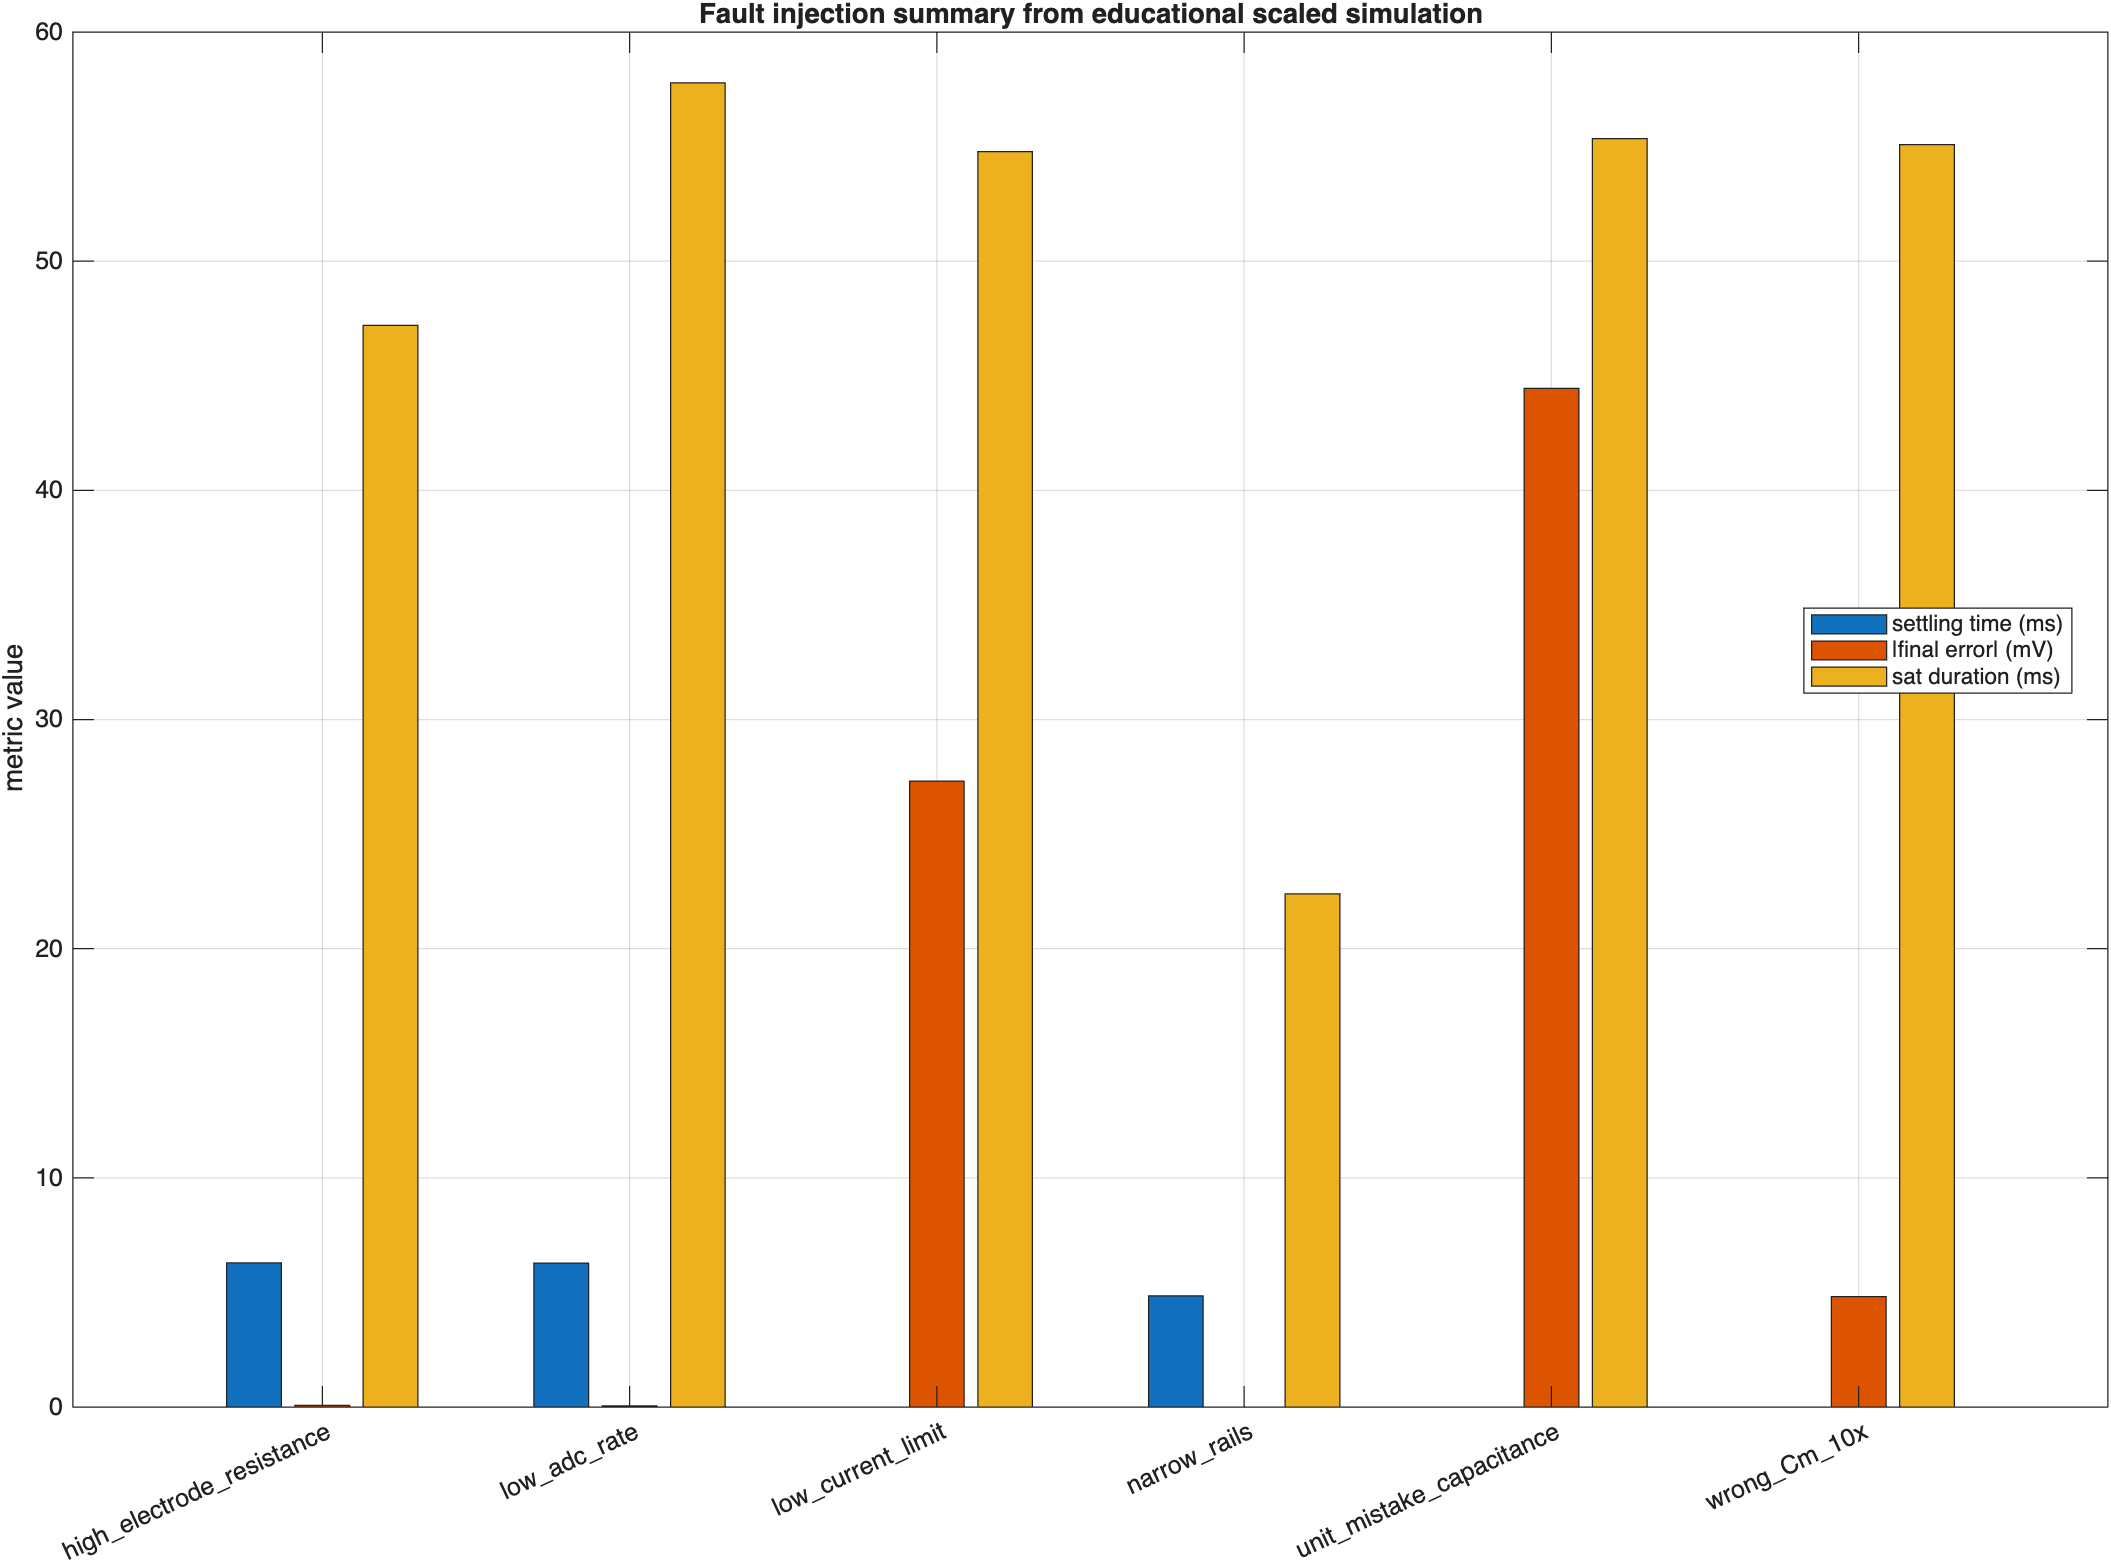
\includegraphics[width=0.47\textwidth]{figures/fig5_mixed_faults.png} \\
(c) ADC/digital logic & (d) Fault summary
\end{tabular}
\caption{Benchmark 3 mixed-signal evidence using educational scaled parameters. The model exposes non-settling, saturation, ADC/digital behavior, and fault sensitivity.}
\label{fig:mixed}
\end{figure*}
